\title{Layout of the PoC}
\textsc{Olav ten Bosch and Michael Schaefer}
\vspace{0.6cm}

In order to do a proof of concept on a common set of validation cases in two different countries it was necessary to agree on the process to follow. For this we developed a process diagram, which is shown in figure \ref{pocprocess}.


\begin{figure}[h!]
\begin{center}
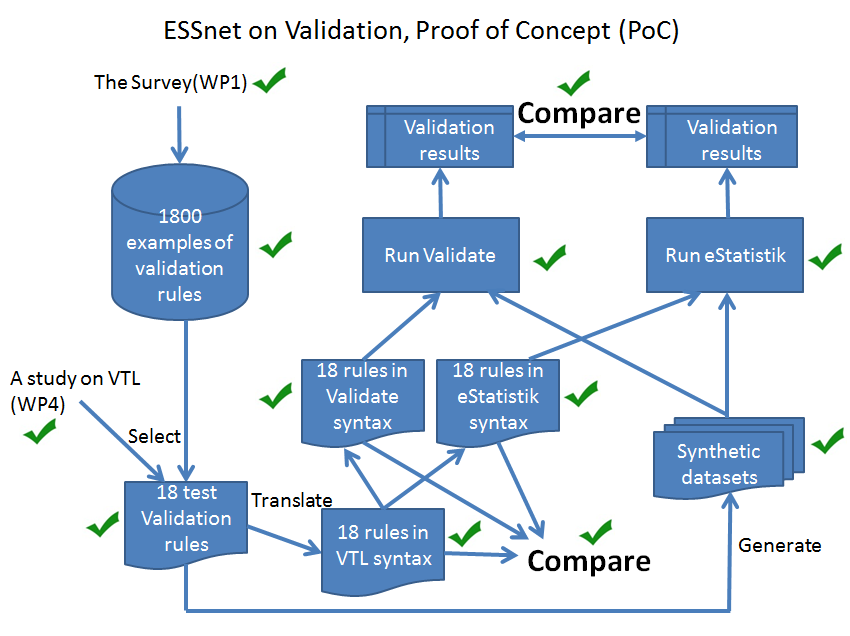
\includegraphics[scale=0.5]{20151207ESSnetPoCProcess.PNG} 
\end{center}
\caption{Process outline of the VTL proof of concept}
\label{pocprocess}
\end{figure}

In a first step, we selected a set of 18 validation rules of varying complexity
to be used in the PoC. Those rules were drawn from two sources:

\begin{itemize}
\item
The repository of about 1800 validation rules collected in the project survey on
data validation in the ESS. Those rules are real-world samples of practically
applied validation rules expressed in a variety of formats (SQL, natural language,
SAS, Blaise, etc.).
\item
The rules mentioned in the "Study on VTL". We have added rules from this study
because they express an interesting variety of possibilities in terms of validation.
\end{itemize}

Next, it was necessary to have data to test the rules against. It would have been
optimal if the PoC could have used real data to work on. Although there existed real
data for the rules drawn from the survey data it would at least have been very hard to get, and
it was outright impossible for the rules originating from the study. Therefore, we
decided to generate synthetic data sets for all 18 rules. It was also decided to
allow for missing values and to specify the expected output of the validation at the
record and data set level. This is explained in more detail in chapter~\ref{datarules}.
Both validation rules and synthetic data sets are available on \citep{GIT:2015}.

The 18 test validation rules were implemented in VTL 1.0 by a VTL expert. At the
NSIs of Germany and the Netherlands a \textit{neutral} person, meaning one not
involved in the ESSnet and unfamiliar with VTL, but experienced in programming
and the national validation systems, was assigned to the task of translating
the VTL rules into the respective national specification language. This person
was asked to use only the VTL code and the data set definitions as a starting
point and not to resort to the natural language descriptions of the rules or
external expertise as far as he or she could avoid. This request was made to
better emulate the use of VTL as a communication language for international
and national organisations.

This resulted in implementations of the rules in the \textit{eSTATISTIK} and
\textit{Validate} languages. These implementations were then used in their
respective runtime environments to validate the synthetic data sets . In a last
step, the validation results and the three implementation flavours (\textit{VTL},
\textit{eSTATISTIK}, \textit{Validate}) were compared.

